\section{Simulações}

Simulações foram realizadas para testar os dispositivos projetados. Os testes avaliaram o funcionamento geral do circuito de acordo com as especificações do projeto, e também o funcionamento dos componentes APS e TIA.

Para a realização das simulações, é necessário se realizar uma estimativa da fotocorrente gerada dos fotodiodos. Como até o momento da simulação não havia a disponibilidade de uma amostra do fotodiodo utilizado, o autor fez uma estimativa conforme o trabalho de \cite{LidianeCampos}, apresentado na \autoref{tab_estcur}.

\begin{table}[htbp]
\caption{Estimativa de faixa de fotocorrente gerada}
\label{tab_estcur}
\centering
\begin{tabular}{cc}
\toprule
& Corrente nA \\
\midrule \midrule
Mínimo & 0,1\\
\midrule
Maximo & 30\\
\bottomrule
\end{tabular}
\legend{Fonte: Produzido pelo autor baseado no trabalho \cite{LidianeCampos}}
\end{table}

\subsection{Máximo sinal DC do APS}
\label{DCAPS}

É avaliado qual é o sinal DC que o bloco APS apresenta sem ter nenhuma fotocorrente gerada, $T_{enable}$ desabilitado e $T_{reset}$ habilitado. Na situação $V_{cn}$ irá apresentar o valor de VDD, o que vai representar o máximo sinal possível em $V_{out}$. A corrente \textit{Iref} considerada foi de $500$ nA, fornecida pelo bloco \textit{current\_mirror\_nmos}. Uma carga de $100$ fF foi utilizada na saída do APS de forma a simular a conexão com  um transistor na saída. O valor obtido foi de $1,15813$ V para $V_{out}$.

\subsection{Máximo sinal DC do APS no APS\_digitalized}

É avaliado qual é o sinal DC que o bloco APS conectado a um comparador apresenta sem ter nenhuma fotocorrente gerada, $T_{enable}$ desabilitado e $T_{reset}$ habilitado. Na situação $V_{cn}$ irá apresentar o valor de VDD, o que vai representar o máximo sinal possível em $V_{out}$. A corrente \textit{Iref} utilizada para a simulação foi de $500$ nA, fornecida pelo bloco \textit{current\_mirror\_nmos}. Uma carga de $100$ fF foi utilizada na saída do APS de forma a simular outras capacitâncias que podem aparecer no nó. O valor obtido foi de $1,15813$ V para $V_{out}$, equivalente ao apresentado na \autoref{DCAPS}.

\subsection{Máximo sinal DC do APS no APS\_digitalized}

É avaliado qual é o sinal DC que o bloco APS conectado a um comparador apresenta sem ter nenhuma fotocorrente gerada, $T_{enable}$ desabilitado e $T_{reset}$ habilitado. Na situação $V_{cn}$ irá apresentar o valor de VDD, o que vai representar o máximo sinal possível em $V_{out}$. A corrente \textit{Iref} utilizada para a simulação foi de $500$ nA, fornecida pelo bloco \textit{current\_mirror\_nmos}. Uma carga de $100$ fF foi utilizada na saída do APS de forma a simular outras capacitâncias que podem aparecer no nó. O valor obtido foi de $1,15813$ V para $V_{out}$, equivalente ao apresentado na \autoref{DCAPS}.

\subsection{Análise transiente do sinal de saída}

É avaliado qual a resposta do APS com a presença de uma fotocorrente. Para a simulação, foi considerado o modelo apresentado na \autoref{fig_APS_cap}, do qual há uma fonte de corrente em paralelo a um diodo representando a fotogeração. A corrente \textit{Iref} considerada foi de $500$ nA, fornecida pelo bloco \textit{current\_mirror\_nmos}.

O Período de Reset é sempre definido para ter uma duração de $1$ us, de forma que esse valor precisa ser suficiente para que o sinal em $V_{cn}$ estabilize em VDD (como discutido na \autoref{secao_amostrando}). Dois valores para o Período de Integração foram considerados, como mostrado nas próximas subseções.

\subsection{Período de Integração igual a 121 $\mu$s}

Nessa situação, foi considerado uma fotocorrente de 5 nA, que está dentro da faixa proposta pelo autor na \autoref{tab_estcur}. Os resultados obtidos são observados nos gráficos abaixo.

\begin{figure}[htb]
 \centering
  \begin{minipage}{0.4\textwidth}
    \centering
    \caption{   A}
    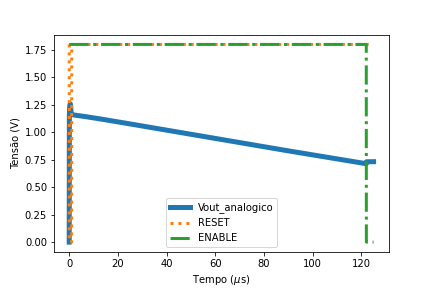
\includegraphics[scale=0.8]{Resultados/Graficos/reseteenable-tb_pixel125.png}
    \legend{Fonte: Produzido pelo autor}
  \end{minipage}
  \hfill
  \begin{minipage}{0.4\textwidth}
    \centering
    \caption{A} 
    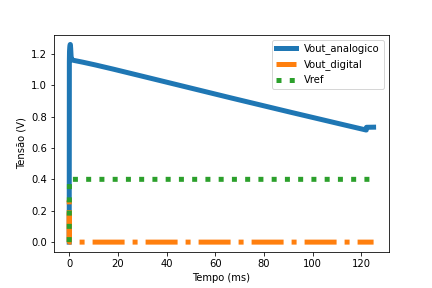
\includegraphics[scale=0.8]{Resultados/Graficos/analogicoedigital-tb_pixel125.png}
    \legend{Fonte: Produzido pelo autor}
  \end{minipage}
\end{figure}

\subsection{Período de Integração igual a 121 $\mu$s}